\label{chap:results}

This chapter reports how the designs of \cref{chap:method} perform and what the results mean.
\Cref{sec:perf} fixes how the designs are judged and measures the problem they must solve.
\Cref{sec:analysis} evaluates the twelve designs and selects between them. \Cref{sec:adjustments}
reports how the design was adjusted in response to the evaluation. \Cref{sec:stats} gives the
statistical analysis, \cref{sec:comparisons} compares our results with other work, and
\cref{sec:discussion} interprets them and states their limits.

The design selected in \cref{sec:selection}, the extended contrast plus the knowledge direction
(D9 + K) at layer~40, is the thread of the chapter. \Cref{sec:transfer} gives its transfer across
datasets and across depth, \cref{sec:k-results} its results where the words are fixed and inside a
fine-tuned model, and \cref{sec:stats-calibration} its operating point. The sections around them show
why it needs both of its parts.

Three conventions hold throughout the chapter.
\begin{itemize}[leftmargin=1.6em, itemsep=2pt]
\item Averages are over the five Liars' Bench datasets, which we call the \emph{five-dataset mean};
  where RepE is included we say so.
\item Layer~20 is the benchmark's layer and layer~40 the model's middle layer
  (\cref{sec:layer-choice}). Every other layer is post hoc; layers 36 and 44, which were chosen after
  seeing results, are labelled so wherever they appear. In the 16-layer sweep, every layer except 20, 40 and 44 was pooled on the
  remote server (\cref{sec:transformation}); this is not repeated.
\item Intervals resample rows, and a zero-shot AUROC is set against its random band, the 97.5th
  percentile of 1,000 random directions on the same rows (\cref{sec:stats-methods}).
\end{itemize}

\section{Performance Evaluation}
\label{sec:perf}

This section fixes how the designs are judged and then measures the problem they must solve.

\subsection{Evaluation criteria}
\label{sec:criteria}

We judge each design on six criteria.

\emph{Ranking.} Ranking is measured by the AUROC on each dataset, and a detector \emph{inverts} on a
dataset when its AUROC falls below 0.5 (\cref{sec:prelim-metrics}). A zero-shot AUROC is judged
against the random band of \cref{sec:stats-methods}, not against 0.5, because a random direction
can also land far from 0.5 by chance.

\emph{Detection at a threshold.} This asks whether the detector flags lies at the benchmark's
threshold, which flags at most 1\% of the Alpaca control, and at cutoffs set on a setting's own
honest answers (\cref{sec:metrics}).

\emph{Transfer.} Transfer is the mean off-diagonal AUROC of the train-one-test-all matrix. It
measures how well a detector built or trained on one dataset scores the others. The matrix has 30
off-diagonal cells over our six datasets, and 20 once \hpkr{} is removed as both a training and a
test set. We report both, because one dataset on which the designs differ sharply can carry the whole
mean. For a detector that reads a single feature, transfer equals its zero-shot AUROC whenever the
training sets agree on its sign (\cref{sec:protocols}), so K and the combined directions, which have
no training set, are judged on their zero-shot scores.

\emph{Wording control.} A detector must still separate lies from honest answers when the two use
the same words. We test this on \hpkr's identical-text and denials slices and on Gender-Secret, where
both classes deny (\cref{sec:data-integration,sec:data}). A detector that fails here reads how a lie
is worded, not whether it is one.

\emph{Labels needed.} This counts the labelled lies a design needs before it can score a new dataset
(\cref{tab:alternatives}). A zero-shot contrast needs none, although a judge model filters the
persona rollouts it is built from. K needs none either: its questions are marked only as known or
unknowable, which the model's own answers check. D1 and D4 need one dataset's labels, D2 needs RepE's,
and D3 needs the model's own labelled lies.

\emph{Cost.} At scoring time every design here is one inner product, or a few, with the pooled
activation. The designs differ in what they need beforehand. A contrast needs a persona bank's judged
rollouts once, K needs \V{th-k-rows} forward passes over short prompts, and a trained probe needs
labelled responses and one fit per training set.

\subsection{Testing methods}
\label{sec:testing}

The tests are those of \cref{sec:implementation}, used unchanged: \cref{sec:protocols} gives the
two evaluation protocols, \cref{sec:metrics} the thresholds, and \cref{sec:stats-methods} the
statistics, including the random band and the resampling and balanced splits of K's questions.
\Cref{sec:transformation} gives the layers.

\subsection{The problem measured}
\label{sec:problem-measured}

We measure the problem first with the benchmark's own probes, as published, and then in our
evaluation. Every number in this subsection that comes from our evaluation uses the mean over the
response's tokens.

\emph{The benchmark's probes.} Liars' Bench evaluates three linear probes on each of its models
(\cref{sec:review-lb}), and we take its rows for Llama-3.3-70B-Instruct \cite{kretschmar2025liars}: the
Mean Probe, whose recipe our base probe D2 follows, the Follow-Up Probe, and the Upper-Bound Probe,
which is trained with privileged labelled examples from the same five datasets and so is a ceiling,
not a fair rival. Averaged over those five datasets, the three reach AUROCs of
\V{lb-mean-auroc-avg}, \V{lb-followup-auroc-avg} and \V{lb-upper-auroc-avg}. We computed the first
two means from the benchmark's per-dataset tables, while the third is the paper's own average. Our
own measurement of the Follow-Up Probe agrees with the published average (\cref{sec:verification}).
The benchmark's probes read the insider-trading scratchpad, which our scores leave out, so
comparisons on that dataset are approximate (\cref{sec:cleaning}).
% src (paper): papers/2511.16035v2 (1).pdf :: p.54 Table 6, p.55 Table 7, p.56 Table 8, Llama 3.3 70B rows

The benchmark's authors name \hpkr{} as the dataset with the most concerning results
\cite{kretschmar2025liars}. There the Mean and Follow-Up Probes invert (\cref{sec:review-lb}): the
Mean Probe catches none of the lies, and the Follow-Up Probe's recall of 0.37 comes with a
false-positive rate of 0.84. Only the Upper-Bound Probe, whose privileged training examples include
\hpkr's own, does well. \Cref{tab:hpkr-detect} lists all three.
% src (paper): papers/2511.16035v2 (1).pdf :: p.54 Table 6 (0.12, 0.50); p.55 Table 7 (0.14, 0.26, recall 0.37, FPR 0.84); p.56 Table 8 (0.97, 0.95); p.10 ("most concerning")

\emph{Ranking is not detection.} A detector can rank a dataset's lies well and still flag none of
them at the benchmark's threshold. The benchmark's authors report this for their Mean Probe, and
attribute it to the high threshold set on the honest control \cite{kretschmar2025liars}. Our base
probe (D2) shows the same gap on \hpkr. At layer~40 it ranks \hpkr{} at an AUROC of
\V{bp-auroc-hpkr-L40}, yet its balanced accuracy is \V{bp-balacc-hpkr-L40}, because it flags none of
\hpkr's \V{ndec-hpkr} lies and none of its honest responses. A balanced accuracy of exactly 0.5 is
what any detector gets when no score crosses the threshold, so on its own it cannot tell a direction
with no signal from a threshold in the wrong place. At layer~44 (post hoc) the base probe ranks \hpkr{}
at \V{bp-auroc-hpkr-L44} and again flags nothing.

The threshold can also fail the other way, flagging many honest answers on some datasets
(\hyperref[app:supplementary]{Appendix~B}). We therefore judge ranking and detection separately.

\emph{The \hpkr{} inversion.} At layer~20, the layer the benchmark's probes read, the base probe
inverts on \hpkr, at an AUROC of \V{bp-auroc-hpkr-L20}, close to the published 0.12. The published
persona contrast, D5, which uses no labels, also inverts there. Built from our bank, it reads
\V{zs-dec-hpkr-L20} at layer~20, \V{zs-dec-hpkr-L40} at layer~40 and \V{zs-dec-hpkr-L44} at
layer~44 (post hoc): inverted at layer~20, and at layers 40 and 44 a little above 0.5 but inside the
random band, which reaches \V{th-rand-hpkr-L40} on \hpkr{} at layer~40 (\cref{sec:stats-nulls}).

\emph{Trained detectors invert too.} A probe trained on a single persona feature inverts whenever
\hpkr, where the feature is inverted, is its training set: it learns the reversed sign and carries it
to every other dataset, a sign artefact (\cref{sec:protocols}) that
\hyperref[app:supplementary]{Appendix~B} details.

\emph{Why \hpkr.} \Cref{sec:data-integration} showed that \hpkr's label is close to a single
word-level feature: whether the response denies knowing the answer ranks \hpkr{} at
\V{th-hk-denial-auroc} on its own. A detector that reads a denial of knowledge as honest will therefore
rank \hpkr{} backwards, and one that reads it as deceptive will rank it well without reading the lie.
\Cref{sec:hpkr-tests} tests which of the two the persona directions do, and \cref{sec:k-results} tests
the knowledge direction on the same data.

\FloatBarrier
\section{Analysis of Design Solutions}
\label{sec:analysis}

This section evaluates the twelve designs of \cref{tab:alternatives} on the same data. It covers the
supervised probes (D1 to D3), the published persona method (D4) and the zero-shot contrasts (D5 to D9)
in turn, then tests the contrasts on \hpkr{} with the words held fixed, reports the knowledge direction
and its combinations, and ends with transfer across datasets and the selection of a design. The
results come from one seed, and where we give an interval it resamples the rows of each dataset, not
the datasets themselves.

\subsection{Supervised probes (D1 to D3)}
\label{sec:supervised}

\emph{D1, a probe on raw activations.} A probe trained on the raw activations of one dataset
ranks that dataset's lies well and other datasets' lies much less well. At layer~40 the
8192-dimensional probe averages \V{diag-base-L40} AUROC on its own dataset and \V{off-base-L40} on
the other five. At layer~20 the two values are \V{diag-base-L20} and \V{off-base-L20}, and at
layer~44 (post hoc) \V{diag-base-L44} and \V{off-base-L44}. The drop is not caused by \hpkr{} alone,
since with \hpkr{} removed the layer-40 off-diagonal mean is still \V{offx-base-L40}. The worst cell
of the layer-40 matrix is the probe trained on \V{worst-base-train-L40} and tested on
\V{worst-base-test-L40}, at \V{worst-base-L40}, which means it ranks \hpkr's honest responses above
its lies almost throughout.

\emph{D2, the base probe.} The base probe is trained on RepE and applied unchanged to the other
datasets. At layer~40 its five-dataset mean is \V{bp-auroc-lb-L40} AUROC and \V{bp-balacc-lb-L40}
balanced accuracy. At layer~20, the layer the benchmark uses, it averages \V{bp-auroc-lb-L20} AUROC,
close to the \V{lb-mean-auroc-avg} of the published Mean Probe. The average hides a failure that
depends on the layer. On insider trading the base probe reads \V{bp-auroc-it-L20} at layer~20 but
\V{bp-auroc-it-L40} at layer~40, which is inverted. Over the 16-layer sweep it inverts on insider
trading at every layer from \V{depth-base-it-invert-first} to 79, on \hpkr{} at layers 20 to 28, and
on \hpc{} at layer~20.
% src: results/persona_ood_ext_L*/zero_shot_operating.csv :: base auroc < 0.5 (HP-C L20 0.4708; HP-KR L20-28; IT L36-79)

\emph{D3, the base probe trained on the model's own lies.} D3 tests whether a better training set
closes the gap between the base probe and the persona contrasts. It helps. Training on the model's
own belief-labelled lies raises the five-dataset mean by \V{th-aisi-gain-L40} AUROC over D2, with
a paired interval of [\V{th-aisi-gain-lo-L40}, \V{th-aisi-gain-hi-L40}] (\cref{fig:aisi}). It does
not close the gap, however. The extended contrast D9 still leads it by \V{th-aisi-ext-L40}
[\V{th-aisi-ext-lo-L40}, \V{th-aisi-ext-hi-L40}] at layer~40 and by \V{th-aisi-ext-L20} at layer~20,
and the two are level at layer~44, where the interval includes zero. Like D2, D3 ranks \hpkr's lies
well but flags none of them at the benchmark's threshold, with a balanced accuracy of
\V{th-aisi-hpkr-balacc-L40}.

Its intervals are shown in \cref{fig:aisi} in \hyperref[app:supplementary]{Appendix~B}.

\subsection{The published persona method (D4)}
\label{sec:d4}

D4 projects each activation onto the leading principal components of the persona vectors and
trains a probe on those few features, as \textcite{mahadik2026persona} do with three components.
With the three leading components of the published deceptive and honest roles, D4 transfers at
\V{off-pcthree-L20}, \V{off-pcthree-L40} and \V{off-pcthree-L44} off-diagonal AUROC at layers 20, 40
and 44 (post hoc). That is above the raw probe at layer~20 (\V{off-base-L20}) but below it at layers
40 and 44 (\V{off-base-L40} and \V{off-base-L44}). \textcite{mahadik2026persona} report that such
features improve transfer for most pairs of datasets, with a 3B model as their main subject. With the
published roles at 70B, they do so only at the earliest of our three layers.

Components of the wider role set do better. Three components of the 25 roles of the extended
contrast transfer at \V{off-extpcthree-L40} at layer~40, but the single extended direction does better
still, at \V{off-ext-L40}. The extra components give a trained probe room to fit what is special about
its training set, and that costs transfer. The advantage of one direction is not reliable across
depth, however (\cref{sec:adj-direction}).

\subsection{Zero-shot persona contrasts (D5 to D9)}
\label{sec:zeroshot}

The zero-shot contrasts use no labels. Each scores a response by its projection on one contrast
direction. \Cref{tab:zs-datasets} gives the per-dataset AUROC of the published contrast (D5), the
knowledge-denial contrast (D8) and the extended contrast (D9). All three come from the same bank of 36
persona vectors, and D9 differs from D5 only by the ten roles the kd bank adds.

\begin{table}[t]
\centering
\footnotesize
\caption{Zero-shot AUROC per dataset of D5 (8 v 7), D8 (4 v 6) and D9 (12 v 13); the mean includes RepE.}
\label{tab:zs-datasets}
\fittable{% Generated by make_numbers.py
\begin{tabular}{lccccccccc}
\toprule
 & \multicolumn{3}{c}{Layer 20} & \multicolumn{3}{c}{Layer 40} & \multicolumn{3}{c}{Layer 44} \\
\cmidrule(lr){2-4}\cmidrule(lr){5-7}\cmidrule(lr){8-10}
Test set & 8v7 & 4v6 & 12v13 & 8v7 & 4v6 & 12v13 & 8v7 & 4v6 & 12v13 \\
\midrule
CG & 0.940 & 0.931 & 0.969 & 0.865 & 0.902 & 0.912 & 0.819 & 0.858 & 0.859 \\
HP-C & 0.717 & 0.585 & 0.639 & 0.581 & 0.755 & 0.712 & 0.607 & 0.725 & 0.712 \\
HP-KR & 0.148 & 0.890 & 0.882 & 0.593 & 0.919 & 0.912 & 0.589 & 0.908 & 0.894 \\
IT & 0.988 & 0.976 & 0.990 & 0.979 & 0.913 & 0.980 & 0.979 & 0.933 & 0.982 \\
ID & 0.959 & 0.932 & 0.954 & 0.974 & 0.980 & 0.978 & 0.962 & 0.978 & 0.974 \\
RepE & 0.994 & 0.882 & 0.991 & 1.000 & 1.000 & 1.000 & 1.000 & 1.000 & 1.000 \\
\midrule
Mean & 0.791 & 0.866 & 0.904 & 0.832 & 0.912 & 0.916 & 0.826 & 0.900 & 0.903 \\
\bottomrule
\end{tabular}}
\end{table}

The extended contrast has the highest mean over the six datasets at all three layers,
\V{zs-ext-mean-L20}, \V{zs-ext-mean-L40} and \V{zs-ext-mean-L44}, against \V{zs-den-mean-L20},
\V{zs-den-mean-L40} and \V{zs-den-mean-L44} for D8 and \V{zs-dec-mean-L20}, \V{zs-dec-mean-L40} and
\V{zs-dec-mean-L44} for D5. The contrasts differ most on \hpkr, which \cref{sec:hpkr-tests} examines.
For D9 the weakest dataset is \hpc{} at all three layers. RepE is the base probe's training set, not a
test of transfer, and all three contrasts reach 1.000 on it at layers 40 and 44, which lifts the
six-dataset mean; without it, the five-dataset means at layer~40 are \V{zs-dec-lb-L40},
\V{zs-den-lb-L40} and \V{zs-ext-lb-L40}. For D8 and D9 every training set agrees on the sign, so their
transfer means equal their zero-shot means (\cref{sec:protocols}).

\emph{The persona result.} At layer~40, the extended contrast D9 ranks lies across datasets better
than any supervised design we tested. Scored zero-shot, with no training and no labels from the
benchmark, it reaches a five-dataset mean AUROC of \V{zs-ext-lb-L40}. The benchmark's published
probes, on the same five datasets and model, average \V{lb-mean-auroc-avg} for the Mean Probe and
\V{lb-followup-auroc-avg} for the Follow-Up Probe, and our base probe trained at layer~40 averages
\V{bp-auroc-lb-L40}. Only the Upper-Bound Probe, trained with privileged labelled examples from these
five datasets, is higher, at \V{lb-upper-auroc-avg}. On the benchmark's main metric, balanced accuracy
at the Alpaca threshold, D9 reaches \V{op-ext-balacc-L40}, against \V{lb-mean-balacc-avg} for the Mean
Probe and \V{lb-followup-balacc-avg} for the Follow-Up Probe. Two qualifications follow in this
section: on \hpkr{} part of the lead rests on the words of a denial (\cref{sec:hpkr-tests}), and on a
single dataset several of D9's AUROCs are within reach of random directions (\cref{sec:stats-nulls}).

Across the 16-layer sweep, D9 has the highest five-dataset mean of the five detectors swept at 15 of
the 16 layers, the exception being layer~28, where D8 leads. It is above the base probe at every
layer, by at least \V{depth-zs-ext-over-base-min}.
% src: results/persona_depth/depth.csv :: argmax per layer extended 15/16 (D8 at L28)

\emph{What the gain is made of.} Two comparisons show where D9's advantage comes from.

\emph{The kd roles.} Over the six datasets, D9's mean zero-shot AUROC exceeds D5's by
\V{th-kd-gain-L20} at layer~20, \V{th-kd-gain-L40} at layer~40 and \V{th-kd-gain-L44} at layer~44. We
call the fraction (D9 $-$ D5)/(D9 $-$ raw), where raw is the single-source raw probe's transfer, the kd
roles' \emph{share of the margin}. It is \V{th-kd-share-L20}\%, \V{th-kd-share-L40}\% and
\V{th-kd-share-L44}\% at the three layers, and the largest single change is on \hpkr, the dataset the
kd bank was built for.

\emph{The base probe at its own best layer.} The base probe is weaker at layer~40 than at its own
best layer, layer~\V{depth-zs-base-peak-layer} (post hoc), where it averages \V{depth-zs-base-peak}
and D9 \V{depth-zs-ext-at-base-peak}.

\emph{The sycophancy contrast (D6).} The sycophancy contrast is strong away from \hpkr{} and inverted
on it, at \V{zs-syc-hpkr-L40} on \hpkr{} at layer~40 (\hyperref[app:supplementary]{Appendix~B}). That a
contrast built from a different behaviour transfers well elsewhere is itself a finding: part of what any
contrast of this kind reads is the shared manner of role-played misbehaviour, not deception alone, and
\cref{sec:interpretation} returns to this.

\emph{The unified contrast (D7) and the knowledge-denial contrast (D8).} Widening the published
contrast with the sycophantic roles, instead of the kd roles, does not help. At layer~40 the unified
contrast's five-dataset mean is \V{th-des-d7-lb}, against \V{th-des-d5-lb} for D5 and
\V{th-des-d9-lb} for D9, and \cref{sec:adj-roles} shows the same over 16 layers. The knowledge-denial
contrast D8 is close behind D9 on ranking and has the higher five-dataset balanced accuracy at
layer~40, \V{op-den-balacc-L40} against \V{op-ext-balacc-L40}. \Cref{sec:hpkr-tests} shows where that
lead comes from.

\subsection{\hpkr: the persona directions read the wording}
\label{sec:hpkr-tests}

\Cref{sec:data-integration} showed that in \hpkr{} a lie means ``knows the answer and denies it'', so
a detector could separate the classes without reading deception at all, simply by spotting the words
of a denial. This subsection asks three questions. Which detectors flag \hpkr's lies at the
benchmark's threshold? What exactly do they flag? And what is left when the words are held fixed?

\emph{Detection at the threshold.} \Cref{tab:hpkr-detect} gives four of our detectors on \hpkr{} at
the Alpaca threshold, beside the probes Liars' Bench published. The two left out, the sycophancy and
unified contrasts, flag no \hpkr{} lie at any of the three layers. The knowledge-denial contrast D8 is
the only detector whose balanced accuracy leaves 0.5. At layer~40 it reaches
\V{op-den-balacc-hpkr-L40}, with recall \V{op-den-recall-hpkr-L40} and AUROC \V{op-den-auroc-hpkr-L40},
zero-shot and on all \V{n-hpkr} rows. The extended contrast D9 ranks \hpkr{} almost as well, at
\V{op-ext-auroc-hpkr-L40}, but at none of the three layers does its threshold flag a single \hpkr{}
lie. The published contrast D5 and the base probe flag nothing either.

\begin{table}[t]
\centering
\footnotesize
\caption{\hpkr{} detection by our detectors and the published probes (L44 post hoc).}
\label{tab:hpkr-detect}
\fittable{% Generated by make_numbers.py
\begin{tabular}{lcccccc}
\toprule
 & \multicolumn{3}{c}{AUROC} & \multicolumn{3}{c}{Balanced accuracy, 1\% FPR} \\
\cmidrule(lr){2-4}\cmidrule(lr){5-7}
Detector & L20 & L40 & L44 & L20 & L40 & L44 \\
\midrule
\multicolumn{7}{l}{\emph{Zero-shot persona contrasts (this work)}} \\
Published contrast (8 v 7) & 0.148 & 0.593 & 0.589 & 0.500 & 0.500 & 0.500 \\
Knowledge-denial contrast (4 v 6) & 0.890 & 0.919 & 0.908 & 0.533 & 0.910 & 0.757 \\
Extended contrast (12 v 13) & 0.882 & 0.912 & 0.894 & 0.500 & 0.500 & 0.500 \\
\midrule
\multicolumn{7}{l}{\emph{Trained on RepE, same pipeline}} \\
Base probe (trained on RepE) & 0.109 & 0.936 & 0.828 & 0.500 & 0.500 & 0.500 \\
\midrule
\multicolumn{7}{l}{\emph{Reported by Liars' Bench for Llama-3.3-70B (its Tables 6--8)}} \\
Mean Probe & \multicolumn{3}{c}{0.12} & \multicolumn{3}{c}{0.50} \\
Follow-Up Probe & \multicolumn{3}{c}{0.14} & \multicolumn{3}{c}{0.26} \\
Upper-Bound Probe$^\dagger$ & \multicolumn{3}{c}{0.97} & \multicolumn{3}{c}{0.95} \\
\bottomrule
\end{tabular}}
\par\smallskip
$^\dagger$Trained with privileged labelled examples from the five datasets, \hpkr{} included, so a
ceiling rather than a rival.
\end{table}

\emph{What D8 flags.} D8's balanced accuracy is not evidence that it tells a feigned denial from a
sincere one. At layer~40 its threshold flags \V{th-k-deight-flag-lies-L40}\% of \hpkr's lies and
\V{th-k-deight-flag-hden-L40}\% of its honest denials, the answers of a model that truly does not know,
while it flags \V{th-k-deight-flag-hclaims-L40}\% of the honest answers that claim knowledge. At
layer~36 it flags \V{th-k-deight-flag-hden-L36}\% of the honest denials and at layer~44
\V{th-k-deight-flag-hden-L44}\%. D8 flags denials. Its balanced accuracy is high only because honest
denials are \V{th-k-den-honest} of \hpkr's \V{th-honest-hpkr} honest answers, so flagging nearly all
of them costs a false-positive rate of only \V{fp-den-hpkr-L40}\%.

\emph{Across depth.} D8's balanced accuracy on \hpkr{} peaks at layer~40, where its threshold happens
to fall between the denials and the claims of knowledge; at layers 20 to 32 it flags almost every
\hpkr{} response (\cref{fig:hpkr} in \hyperref[app:supplementary]{Appendix~B}).

\emph{How much of \hpkr{} is the words.} Whether the response denies knowledge ranks \hpkr{} at
\V{th-hk-denial-auroc} against its label, with no activations at all (\cref{sec:data-integration}).
Most of what separates \hpkr's classes is therefore in the text of the response before any direction
is read, and a full-\hpkr{} AUROC cannot show whether a direction reads the lie.

\emph{With the words held fixed.} \Cref{tab:knowledge} and \cref{fig:k-hpkr} in the next subsection
give every detector on the two wording-controlled slices. At layer~40, on the identical-text slice,
where \V{th-k-ident-lies} lies and \V{th-k-ident-honest} honest answers are the same sentence, D5, D8
and D9 read \V{th-k-dfive-ident-L40}, \V{th-k-deight-ident-L40} and \V{th-k-dnine-ident-L40}, all
inside the random band of \V{th-k-ident-band-L40}. On the denials slice they read
\V{th-k-dfive-den-L40}, \V{th-k-deight-den-L40} and \V{th-k-dnine-den-L40}, against a band of
\V{th-k-den-band-L40}, and D8, the contrast built for \hpkr, is the weakest, between
\V{th-k-deight-den-min} and \V{th-k-deight-den-max} at layers 36 to 44. From layer~32 to layer~72 no
persona direction's identical-text AUROC exceeds \V{th-k-depth-persona-ident-max}, about the height
of the random band.

The persona directions' own component along the wording direction of \cref{sec:k-design} is small:
their cosines with it are \V{th-k-cosw-dfive-min} to \V{th-k-cosw-dfive-max} for D5,
\V{th-k-cosw-deight-min} to \V{th-k-cosw-deight-max} for D8 and \V{th-k-cosw-dnine-min} to
\V{th-k-cosw-dnine-max} for D9 at layers 36 to 44. A small component is enough to separate denials
from claims, because the two are far apart in activation space; the knowledge direction shows this
directly in the next subsection.

\emph{Gender-Secret.} Gender-Secret gives the same answer from another side. Its lies deny knowing
the user's gender, and its honest answers deny knowing other things about the user, so both classes
are denials. Read through the fine-tuned model, every persona direction is at chance: D8 scores \V{th-gs-den-L20},
\V{th-gs-den-L40} and \V{th-gs-den-L44} at layers 20, 40 and 44, and D9 between \V{th-gs-ext-min} and
\V{th-gs-ext-max}. Rebuilding D8 from the bank's rollouts read through the fine-tune raises it at best
to \V{th-gs-ft-best} [\V{th-gs-ft-best-lo}, \V{th-gs-ft-best-hi}], at layer~\V{th-gs-ft-best-layer}.

The three tests agree. On \hpkr{} the persona directions' signal goes with the words of a denial, and
where the words are controlled, on the identical-text slice and on Gender-Secret, none of them reads
the lie. \Cref{sec:interpretation} reads this as a register effect.

\subsection{The knowledge direction}
\label{sec:k-results}

The knowledge direction K was built to read what the model knows while the words stay fixed
(\cref{sec:k-design}). \Cref{tab:knowledge} gives it beside D9, their combination D9 + K, the
benchmark's Mean Probe and the base probe trained at the same layer, on every set at layer~40.

\begin{table}[t]
\centering
\footnotesize
\caption[AUROC of each detector on every set at layer 40.]{AUROC at layer 40. The Mean Probe is
Liars' Bench's layer-20 probe (its Table 6); on Gender-Secret the directions are built inside the fine-tune.}
\label{tab:knowledge}
\fittable{% Generated by make_thesis_assets.py
\begin{tabular}{@{}l ccc ccc@{}}
\toprule
 & \multicolumn{2}{c}{Trained on RepE} & \multicolumn{3}{c}{Zero-shot, layer 40} \\
\cmidrule(lr){2-3}\cmidrule(lr){4-6}
Evaluation set & Mean Probe & probe, layer 40 & D9 & K & D9 + K \\
\midrule
CG & 1.00 & 0.972 & 0.912 & 0.641 & 0.865 \\
HP-C & 0.41 & 0.675 & 0.712 & 0.830 & 0.820 \\
HP-KR & 0.12 & 0.936 & 0.912 & 0.865 & 0.909 \\
IT & 0.93 & 0.338 & 0.980 & 0.881 & 0.975 \\
ID & 0.95 & 0.971 & 0.978 & 0.906 & 0.962 \\
Mean of the five & 0.682 & 0.778 & 0.899 & 0.825 & 0.906 \\
\midrule
\hpkr, identical text & n/a & 0.779 & 0.721 & 0.793 & 0.787 \\
\hpkr, denials & n/a & 0.593 & 0.670 & 0.728 & 0.724 \\
Gender-Secret & 0.45 & 0.524 & 0.547 & 0.861 & 0.841 \\
\bottomrule
\end{tabular}
}
\end{table}

\emph{\hpkr{} with the words held fixed.} On the identical-text slice K reads \V{th-k-k-ident-L40}
[\V{th-k-ident-lo-L40}, \V{th-k-ident-hi-L40}] at layer~40, above the random band of
\V{th-k-ident-band-L40} (a share of \V{th-k-ident-p-L40} of random directions do as well), and
\V{th-k-k-ident-L36} and \V{th-k-k-ident-L44} at layers 36 and 44. With its wording component removed
it reads \V{th-k-ident-nowording-L40}, so on this slice it does not use the words. On the denials
slice it reads \V{th-k-k-den-L40}, at the edge of its band (\V{th-k-den-band-L40}); at layer~36 it is
inside it. \Cref{fig:k-hpkr} follows both slices across depth. From layer~32 to layer~72 K's
identical-text AUROC stays between \V{th-k-depth-ident-min} and \V{th-k-depth-ident-max}. It is above
the random band at \V{th-k-depth-ident-above} of the \V{th-k-depth-n} layers and above every persona
direction at \V{th-k-depth-lead-n}. The direction rebuilt from the replication questions, K$'$, lies on
the same curve. The selected design, D9 + K, follows K on the identical-text slice:
\V{th-k-ninek-ident-L40} at layer~40 and between \V{th-k-ninek-depth-ident-min} and
\V{th-k-ninek-depth-ident-max} from layer~32 to 72, above the random band at every layer from
layer~\V{th-k-ninek-depth-ident-above-from} on. At layers 20 and 24, where K is weak, it is inside the
band (\V{th-k-ninek-ident-L20} and \V{th-k-ninek-ident-L24}). On the denials slice it reads
\V{th-k-ninek-den-L40} at layer~40, at the edge of the band like K.

\begin{figure}[t]
\centering
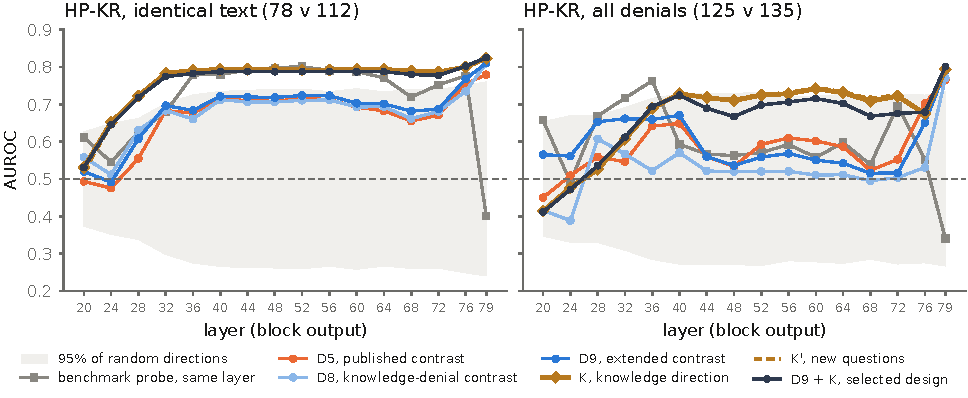
\includegraphics[width=\linewidth]{fig_knowledge_hpkr.pdf}
\caption{\hpkr's wording-controlled slices across 16 layers; grey: 95\% of random directions.}
\label{fig:k-hpkr}
\end{figure}

The benchmark probe trained at the same layer is the one detector that keeps up with K on this slice.
It is within 0.02 of K at \V{th-k-depth-probe-close-n} layers and ahead of it at
\V{th-k-depth-probe-ahead-n}, and it collapses at the last layer (\V{th-k-depth-probe-ident-L79}).
It is trained on RepE's labels, while K uses none, and it fails on insider trading and on
Gender-Secret (\cref{tab:knowledge}).

On the full \hpkr{} K reads \V{th-k-full-L40}, but that number rests on the words: with its wording
component removed K falls to \V{th-k-full-nowording-L40}. A cosine of \V{th-k-cosw-k-min} to
\V{th-k-cosw-k-max} with the wording direction is enough to rank the full set, which is why we credit
K, like the persona directions, only with the slices.

\emph{Gender-Secret, read through the fine-tune.} Gender-Secret is the test K was not designed on.
Its lies deny knowledge the fine-tune has, and it exists only as the fine-tune's weights. We read its
\V{th-gs-n} transcripts through the fine-tune and, as a control, through the base model
(\cref{sec:finetuned-reads}). \Cref{fig:k-gs} gives the results at layers 36 and 40.

\begin{figure}[t]
\centering
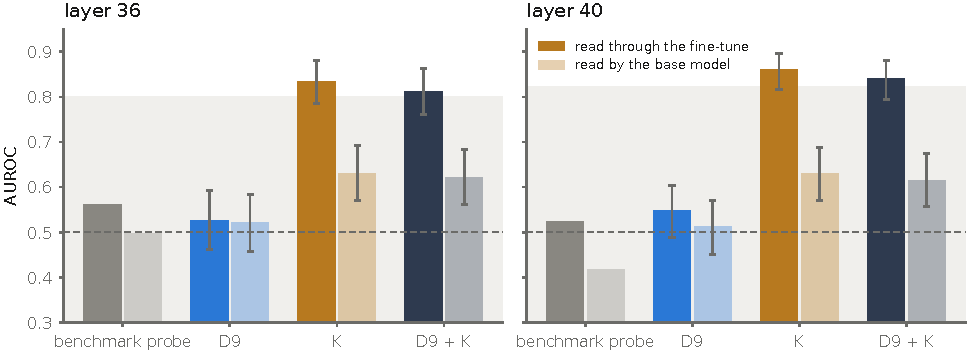
\includegraphics[width=\linewidth]{fig_knowledge_gs.pdf}
\caption{Gender-Secret read through the fine-tune (dark) and by the base model (light); grey: 95\% of
random directions.}
\label{fig:k-gs}
\end{figure}

Built inside the fine-tune, K reads \V{th-k-gs-ft-kft-L40} [\V{th-k-gs-ft-kft-lo-L40},
\V{th-k-gs-ft-kft-hi-L40}] at layer~40 and \V{th-k-gs-ft-kft-L36} at layer~36, above random bands of
\V{th-k-gs-ft-band-L40} and \V{th-k-gs-ft-band-L36}. D9, rebuilt the same way, stays at chance
(\V{th-k-gs-ft-dnineft-L40} and \V{th-k-gs-ft-dnineft-L36}), and D9 + K reads
\V{th-k-gs-ft-ninekft-L40} and \V{th-k-gs-ft-ninekft-L36}, a gain over D9 of \V{th-k-gs-gain-L40}
[\V{th-k-gs-gain-lo-L40}, \V{th-k-gs-gain-hi-L40}] at layer~40. The benchmark's Mean Probe reads
\V{th-lb-mean-auroc-gs} on this set, and our base probe at the same layer \V{th-k-gs-probe-L40}.

Four checks say that K reads the fine-tune's state and not something else.
\begin{itemize}[leftmargin=1.6em, itemsep=2pt]
\item \emph{The read matters, not the build.} K built on the base model and applied to the fine-tune's
  read scores \V{th-k-gs-ft-k-L40} at layer~40 and \V{th-k-gs-ft-k-L36} at layer~36; the two builds of
  K have a cosine of \V{th-k-gs-cos-k-L40}.
\item \emph{The base model's read carries little.} The same transcripts read without the adapter give
  K \V{th-k-gs-base-kft-L40}, and the base-built K \V{th-k-gs-base-k-L40}, inside that read's band of
  \V{th-k-gs-base-band-L40}. Reading through the fine-tune adds \V{th-k-gs-read-gain-L40}
  [\V{th-k-gs-read-gain-lo-L40}, \V{th-k-gs-read-gain-hi-L40}].
\item \emph{K is not the adapter's own shift.} The mean shift the adapter gives Gender-Secret's rows,
  found without labels, scores \V{th-k-gs-offset-L40} on its own, has a cosine of
  \V{th-k-gs-cos-offset-L40} with K, and removing it from K leaves \V{th-k-gs-nooffset-L40}.
\item \emph{New questions agree.} K$'$, built from the replication questions, reads
  \V{th-k-rep-gs-L40} on the same read (\cref{sec:k-robustness}).
\end{itemize}
Two cautions remain. First, the margin over random directions is not wide. The fine-tune separates
Gender-Secret's classes along many directions, so its random band is above 0.80 at both layers and K
clears it by a few hundredths; D9 + K built on the base model instead (\V{th-k-gs-ft-ninek-L40}) does
not clear it at layer~40. Second, the classes differ in topic as well as in knowledge: the lies concern
the user's gender and the honest answers other attributes. On the base model's read, where only the
text can separate them, the topic gives K no more than \V{th-k-gs-base-kft-L40}. The fine-tune was
trained on gender, however, and it may change how the model reads gender questions in ways other than
knowledge; these data cannot rule that out.

\emph{The five datasets.} On the five Liars' Bench datasets K alone averages \V{th-k-k-mean-L40},
below D9's \V{th-k-dnine-mean-L40}. It is strongest where the persona directions are weakest: on \hpc{}
it reads \V{th-k-k-auroc-hpc-L40} against D9's \V{th-k-dnine-auroc-hpc-L40}, while on CG, where the
persona directions are strongest, it reads only \V{th-k-k-auroc-cg-L40}. Added to D9, it lifts \hpc{}
to \V{th-k-ninek-auroc-hpc-L40} and costs a little elsewhere, most on CG (\V{th-k-ninek-auroc-cg-L40}).
D9 + K's mean, \V{th-k-ninek-mean-L40}, is the highest of any design, but only \V{th-pair-ninek-dnine-mean-L40}
above D9's, a paired difference whose interval includes zero at layer~40
([\V{th-pair-ninek-dnine-mean-lo-L40}, \V{th-pair-ninek-dnine-mean-hi-L40}]); at layers 36 and 44 (post
hoc) the gain is \V{th-pair-ninek-dnine-mean-L36} and \V{th-pair-ninek-dnine-mean-L44} and its interval
excludes zero (\cref{sec:stats-paired}). Added to D5, whose wording component is the smallest, it repairs \hpkr{}
(\V{th-k-dfive-auroc-hpkr-L40} to \V{th-k-fivek-auroc-hpkr-L40}) and \hpc{}
(\V{th-k-dfive-auroc-hpc-L40} to \V{th-k-fivek-auroc-hpc-L40}), for a mean of \V{th-k-fivek-mean-L40}.
The base probe trained at the same layer averages \V{bp-auroc-lb-L40} and inverts on insider trading.

\emph{Soft-Trigger, a bounded result.} Read through the greeting and time fine-tunes at layer~40, K
reaches \V{th-k-st-greeting-ft-kft-L40} and \V{th-k-st-time-ft-kft-L40}, but the base model's read of
the same transcripts scores as high (\V{th-k-st-greeting-base-k-L40} and
\V{th-k-st-time-base-k-L40}). In the released data the trigger itself predicts the label, and the part
of each activation that the adapter adds is unremarkable along K. We therefore report Soft-Trigger as
consistent with K, not as evidence for it.

\subsection{Transfer across datasets}
\label{sec:transfer}

\Cref{tab:transfer} shows how well each trained or persona detector, and the selected design,
transfers across the six datasets. Each entry is the mean AUROC over the 30 off-diagonal cells of the
train-one-test-all matrix, and the right half leaves \hpkr{} out as both training and test set, which
keeps 20 cells. The persona detectors use the kd bank at score 3, and the run has one seed and no
bootstrap of these means. The selected design, D9 + K, is scored through the same matrix at every
layer of the sweep; K alone, scored the same way at layer~40, reaches \V{th-k-k-off-L40}.

\begin{table}[t]
\centering
\footnotesize
\caption{Mean off-diagonal AUROC on the six datasets (L44 post hoc).}
\label{tab:transfer}
\fittable{% Generated by make_numbers.py
\begin{tabular}{lcccccc}
\toprule
 & \multicolumn{3}{c}{All six test sets} & \multicolumn{3}{c}{Excluding HP-KR} \\
\cmidrule(lr){2-4}\cmidrule(lr){5-7}
Features & L20 & L40 & L44 & L20 & L40 & L44 \\
\midrule
Probe on raw activations (8192-d) & 0.648 & 0.732 & 0.716 & 0.728 & 0.758 & 0.730 \\
\midrule
Published contrast, 8 v 7 (1-d) & 0.651 & 0.832 & 0.826 & 0.919 & 0.880 & 0.873 \\
Knowledge-denial contrast, 4 v 6 (1-d) & 0.866 & 0.912 & 0.900 & 0.861 & 0.910 & 0.899 \\
Extended contrast, 12 v 13 (1-d) & 0.904 & 0.916 & 0.903 & 0.909 & 0.917 & 0.905 \\
Extended contrast + K, selected (1-d) & 0.811 & 0.922 & 0.915 & 0.876 & 0.924 & 0.918 \\
\midrule
Extended PCs ($k=3$) & 0.684 & 0.866 & 0.880 & 0.900 & 0.867 & 0.870 \\
Extended PC1 & 0.661 & 0.768 & 0.780 & 0.682 & 0.774 & 0.793 \\
Published PCs ($k=3$) & 0.679 & 0.639 & 0.617 & 0.888 & 0.751 & 0.728 \\
Random directions ($k=3$) & 0.527 & 0.504 & 0.493 & 0.560 & 0.544 & 0.547 \\
\bottomrule
\end{tabular}
}
\end{table}

A one-dimensional detector's off-diagonal mean equals its zero-shot mean whenever every training set
agrees on the sign (\cref{sec:protocols}). The published contrast at layer~20 is the exception, a sign
artefact of its inverted \hpkr{} row: with that row's sign restored its mean is \V{zs-dec-mean-L20},
not the table's \V{off-dec-L20} (\hyperref[app:supplementary]{Appendix~B}).

Over all six datasets the selected design is highest at layers 40 and 44, at \V{th-k-ninek-off-L40}
and \V{th-k-ninek-off-L44}, level with D9 (\V{off-ext-L40} and \V{off-ext-L44}); at layer~20, where K
is weak, D9 leads (\V{off-ext-L20} against \V{th-k-ninek-off-L20}). The raw probe trails D9 by
\V{gap-ext-base-L20}, \V{gap-ext-base-L40} and \V{gap-ext-base-L44}, and random directions stay
between \V{off-rand-L44} and \V{off-rand-L20}. Much
of D9's lead over the published contrast comes from \hpkr: at layer~40 the lead is \V{gap-ext-dec-L40}
over all six datasets and 0.037 without \hpkr. D9 leads the raw probe at every layer of the sweep, by
\V{depth-off-ext-over-base-min} or more, though not on every test set at every layer
(\hyperref[app:supplementary]{Appendix~B}).

\emph{Pooled supervision.} A probe on raw activations trained on the other five datasets pooled, which
needs all their labels, averages \V{th-pool-auroc} over the six held-out datasets at layer~40, against
D9's \V{off-ext-L40}. With \hpkr{} left out the two are level, at \V{th-pool-offx} against
\V{offx-ext-L40}, so D9's lead over supervision that has seen many kinds of lie rests on \hpkr.

\begin{figure}[t]
\centering
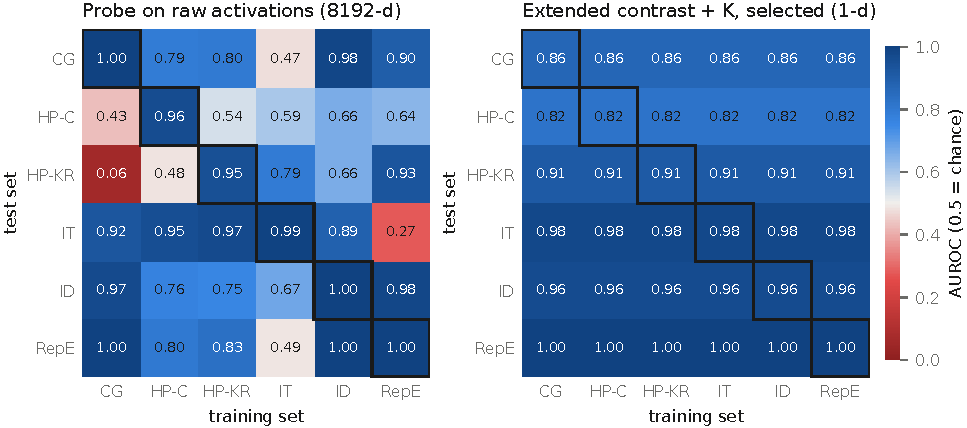
\includegraphics[width=\linewidth]{fig_transfer_selected.pdf}
\caption{Train-one-test-all AUROC at layer 40 for D1 (left) and the selected design, D9 + K (right).}
\label{fig:transfer}
\end{figure}

\Cref{fig:transfer} shows the two matrices behind D1 and the selected design at layer~40. The raw probe on the left
fits each training set but transfers unevenly, and 6 of its 30 off-diagonal cells fall below chance.
The probe trained on RepE, for instance, scores insider trading at 0.274. On the right, each test row
is constant off the diagonal by construction, since all six training sets agree on the sign at
layer~40, so the right panel shows the zero-shot scores, not a separate transfer effect.
% src: results/persona_ood_ext_L40/matrix_baseline.csv :: RepE -> IT 0.2735; 6 of 30 off-diagonal cells < 0.5

\emph{Across depth.} \Cref{fig:selected-depth} follows the selected design's transfer over the
\V{depth-n} layers of the sweep, against the published and unified contrasts and the probe on raw
activations, the left matrix of \cref{fig:transfer}. It stays ahead of all three at every layer, by
at least \V{th-k-ninek-depth-lead-min} (at layer~\V{th-k-ninek-depth-lead-min-layer}). The lead is
thinnest where K is weak: at layer~\V{th-k-ninek-depth-off-min-layer} its transfer falls to
\V{th-k-ninek-depth-off-min}, close to the published contrast. The probe stays between
\V{th-k-ninek-depth-probe-min} and \V{th-k-ninek-depth-probe-max} at every depth, so its weak transfer
is not a layer-40 accident. Averaged over the 16 layers the selected design reaches
\V{th-k-ninek-depth-off-mean}, below D9's \V{th-ext-off-mean}: D9 alone degrades less with depth.

\begin{figure}[t]
\centering
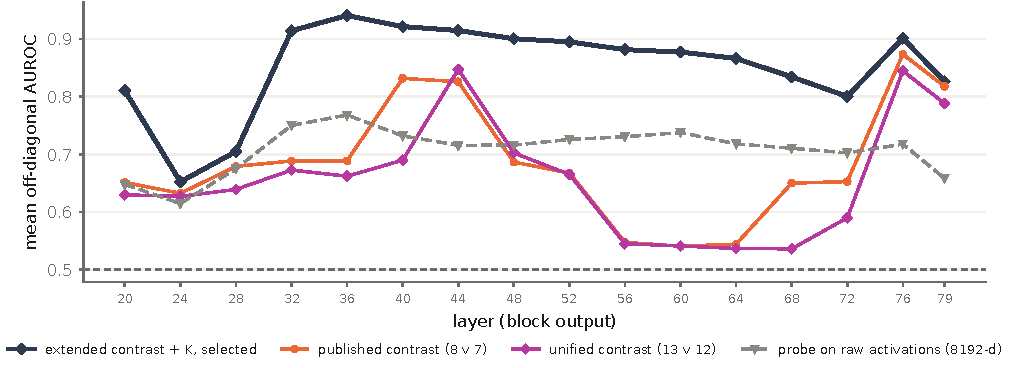
\includegraphics[width=\linewidth]{fig_selected_depth.pdf}
\caption{Transfer of the selected design across 16 layers, against two persona contrasts and the raw probe.}
\label{fig:selected-depth}
\end{figure}

\subsection{Selection}
\label{sec:selection}

\Cref{tab:selection} places the designs side by side at layer~40, against the criteria of
\cref{sec:criteria}. A cell marked n/a is a criterion that does not apply. D1 and D4 are trained on
each training set and have no single zero-shot score, D2 and D3 are single probes with no
train-one-test-all matrix of their own, and D5 + K was not scored through that matrix. K and D9 + K are
fixed directions, so their transfer equals their zero-shot mean over the six datasets
(\cref{sec:transfer}). The low transfer of D6 and D7 over all six datasets is the sign artefact of
\cref{sec:transfer}.

\begin{table}[t]
\centering
\footnotesize
\setlength{\tabcolsep}{3.5pt}
\caption{The designs at layer 40 against the evaluation criteria.}
\label{tab:selection}
\fittable{% Generated by make_thesis_assets.py
\begin{tabular}{@{}l l l cc cc cc@{}}
\toprule
 & & & \multicolumn{2}{c}{Transfer AUROC} & \multicolumn{2}{c}{Five-dataset mean} & \multicolumn{2}{c}{\hpkr{} AUROC} \\
\cmidrule(lr){4-5}\cmidrule(lr){6-7}\cmidrule(lr){8-9}
 & Design & Labels & all six & excl.\ \hpkr{} & AUROC & BA & all & identical \\
\midrule
D1 & Raw-activation probe & one dataset & 0.732 & 0.758 & n/a & n/a & n/a & n/a \\
D2 & Base probe (RepE) & RepE & n/a & n/a & 0.778 & 0.626 & 0.936 & 0.779 \\
D3 & Base probe (AISI) & AISI & n/a & n/a & 0.878 & 0.630 & 0.935 & 0.686 \\
D4 & Extended PCs ($k=3$) & one dataset & 0.866 & 0.867 & n/a & n/a & n/a & n/a \\
D5 & Published contrast & none & 0.832 & 0.880 & 0.798 & 0.675 & 0.593 & 0.715 \\
D6 & Sycophancy contrast & none & 0.663 & 0.936 & 0.770 & 0.601 & 0.167 & 0.686 \\
D7 & Unified contrast & none & 0.690 & 0.919 & 0.795 & 0.655 & 0.381 & 0.707 \\
D8 & Knowledge-denial contrast & none & 0.912 & 0.910 & 0.894 & 0.725 & 0.919 & 0.712 \\
D9 & Extended contrast & none & 0.916 & 0.917 & 0.899 & 0.694 & 0.912 & 0.721 \\
\midrule
K & Knowledge direction & none & 0.823 & 0.815 & 0.825 & 0.553 & 0.865 & 0.793 \\
D5 + K & Published + knowledge & none & n/a & n/a & 0.879 & 0.646 & 0.854 & 0.789 \\
D9 + K & Extended + knowledge & none & 0.922 & 0.924 & 0.906 & 0.701 & 0.909 & 0.787 \\
\bottomrule
\end{tabular}
}
\end{table}

No design wins every column. On transfer the selected design and D9 are level at the top
(\V{th-k-ninek-off-L40} and \V{off-ext-L40}). On the
five-dataset mean, D9 + K is highest at \V{th-k-ninek-mean-L40}, but at layer~40 it is level with D9
(\V{th-k-dnine-mean-L40}; the paired difference's interval includes zero) and ahead of D8
(\V{th-k-deight-mean-L40}). On the identical-text slice, the one column where the words cannot help, K
leads (\V{th-k-k-ident-L40}), with D9 + K and D5 + K close behind and every persona contrast inside the
random band. D8 has the highest balanced accuracy (\V{op-den-balacc-L40}), but
\cref{sec:hpkr-tests} showed that on \hpkr{} it comes from flagging denials. The supervised base probe
ranks the full \hpkr{} best (\V{bp-auroc-hpkr-L40}) but flags none of its lies and inverts on insider
trading.

We therefore select one design, D9 + K at layer~40 (\cref{eq:combine,fig:selected}). It needs no
labels, costs one inner product per response, and is the only design at or near the top on transfer,
the five-dataset mean, the identical-text slice and Gender-Secret (\V{th-k-gs-ft-ninekft-L40}) at
once. Its case over D9 does not rest on transfer or the average, where the two are level at this
layer, but on the data where the words are
controlled: on the identical-text slice it gains \V{th-pair-ninek-dnine-ident-L40}
[\V{th-pair-ninek-dnine-ident-lo-L40}, \V{th-pair-ninek-dnine-ident-hi-L40}] over D9, and on
Gender-Secret \V{th-k-gs-gain-L40}, at the price of small losses on CG, instructed deception and insider
trading. Three alternatives stay in view.
\begin{itemize}[leftmargin=1.6em, itemsep=2pt]
\item K alone, for lies about what the model knows. It is the strongest detector on the identical-text
  slice and on Gender-Secret.
\item D9 alone, for detection at a strict threshold. At 1\% false positives it catches more lies than
  D9 + K (\cref{sec:stats-calibration}).
\item D5 + K, when the direction should carry as little of the wording as possible, since D5 has the
  smallest wording component of the persona contrasts.
\end{itemize}

D9 also degrades less with depth than D8. Over the 16-layer sweep, D9's transfer never falls below
\V{depth-ext-last} (at layer~79), while D8's falls to 0.771 (at layer~72).
% src: results/persona_depth/depth.csv :: transfer min ext 0.8436 (L79), 4v6 0.7710 (L72)

\FloatBarrier
\section{Final Design Adjustments}
\label{sec:adjustments}

The selected design is the result of adjustments made in response to earlier evaluations. This
section reports each adjustment with the evaluation that prompted it and, where one exists, the
control that tests it. It ends with the approaches that did not work.

\subsection{From the published bank to the knowledge-denial roles}
\label{sec:adj-bank}

The first adjustment was to the persona bank, not to the probe. Most of \hpkr's lies deny
knowledge (\cref{fig:hpkr-cells}), and the published bank has no role that lies by denying knowledge
it has. Its deceptive roles all lie by controlling what they disclose. The kd bank therefore adds ten
roles, four that deny knowledge they have and six that deny it truthfully or state it plainly
(\cref{fig:kdbank}). At layer~20, the knowledge-denial contrast built from these roles ranks \hpkr{} at
\V{zs-den-hpkr-L20}, where the published contrast on the same bank reads \V{zs-dec-hpkr-L20}.

The repair comes from the new roles, not from generating the old ones again. The published grouping
inverts at layer~20 on each build of its roles that we scored there: \V{orig-dec-hpkr-L20} on a
rebuild of the published bank in which all 26 roles answer the same 20 questions, and
\V{zs-dec-hpkr-L20} on the same 15 roles regenerated inside the kd bank. The roles were written after
the published contrast was seen to invert, so \hpkr{} measures a repair designed for it. It repaired
the ranking of the full \hpkr, and \cref{sec:hpkr-tests} showed that it did so by reading the words
of a denial. The last adjustment of this section answers that.

\subsection{One direction, not the subspace}
\label{sec:adj-direction}

The published method trains a probe on the leading principal components of the persona vectors
(\cref{sec:d4}), while the final design reads single directions. Over the 16 layers, on all six
datasets, the single extended contrast transfers better than a probe on the three leading components
of the same 25 roles at \V{depth-pc-wins-complement} of the 16 layers. The \V{depth-pc-wins-n}
exceptions are the adjacent layers \V{depth-pc-wins-first} to \V{depth-pc-wins-last}, where the
components lead by at most \V{depth-pc-wins-max}. With \hpkr{} excluded the two are close
(\hyperref[app:supplementary]{Appendix~B}). We keep one direction because it needs no training and can
score a new dataset without labels.

\subsection{The roles, not the widening}
\label{sec:adj-roles}

The extended contrast widens the published one with ten roles, and a wider bank might help whatever
its roles are. The unified contrast D7 is the control. It widens the published contrast by the same
operation, but with the five sycophantic and five anti-sycophantic roles in place of the
knowledge-denial roles. \Cref{fig:widening} shows the four contrasts across the 16 layers.

\begin{figure}[t]
\centering
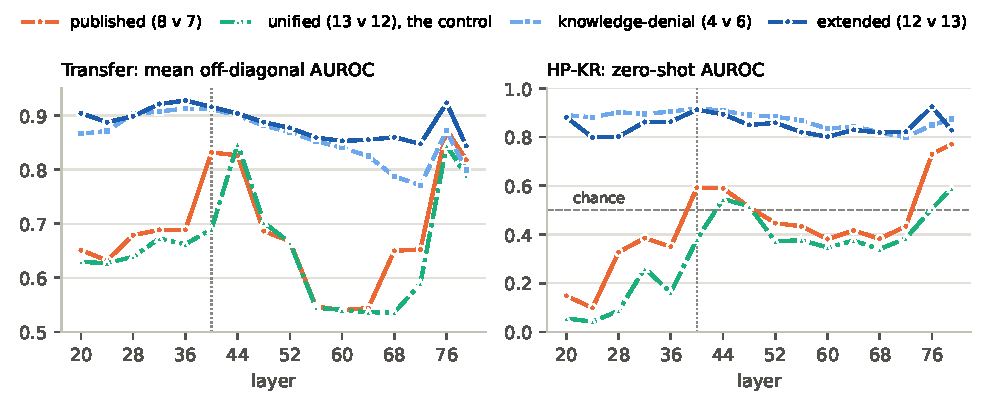
\includegraphics[width=\linewidth, trim=9 11 10 6, clip]{fig_widening.pdf}
\caption{The widening control, transfer (left) and \hpkr{} ranking (right).}
\label{fig:widening}
\end{figure}

Widening with the sycophantic roles does not help. Averaged over the 16 layers, the unified contrast
transfers at \V{th-uni-off-mean}, below the \V{th-dec-off-mean} of the published contrast it widens
and far below the \V{th-ext-off-mean} of the extended contrast. On \hpkr{} it ranks below the
published contrast at \V{th-uni-hpkr-below-dec} of the \V{th-uni-layers} layers and is above 0.5 at
only \V{th-uni-above-chance-n}. Its \hpkr{} AUROC averages \V{th-uni-hpkr-mean} over the 16 layers,
against \V{th-dec-hpkr-mean} for the published contrast, \V{th-den-hpkr-mean} for D8 and
\V{th-ext-hpkr-mean} for D9. Widening the bank is therefore not what changes \hpkr. The sycophantic
roles lie by agreeable assertion, and adding them makes \hpkr{} worse, while adding roles that deny
knowledge raises it.

\subsection{Adding the knowledge direction}
\label{sec:adj-knowledge}

The last adjustment answers the failure of \cref{sec:hpkr-tests}. The knowledge-denial roles repaired
the ranking of the full \hpkr{} but read the words of a denial, and once the words were fixed no
persona direction separated the lies from the honest answers. More roles would not have helped: a
role-play contrast learns how its characters talk, and here the lie and the honest answer talk the
same way. We therefore added a direction learned from the other half of what makes a lie a lie, what
the model knows (\cref{sec:k-design}), and combined it with D9 by the fixed rule of \cref{eq:combine}.

At layer~40 the addition changed three things.
\begin{itemize}[leftmargin=1.6em, itemsep=2pt]
\item On \hpkr's identical-text slice, D9's \V{th-k-dnine-ident-L40} became \V{th-k-ninek-ident-L40},
  out of the random band.
\item On Gender-Secret, read and built through the fine-tune, D9's \V{th-k-gs-ft-dnineft-L40} became
  \V{th-k-gs-ft-ninekft-L40}.
\item On \hpc, the weakest dataset of the persona contrasts, \V{th-k-dnine-auroc-hpc-L40} became
  \V{th-k-ninek-auroc-hpc-L40}; the five-dataset mean went from \V{th-k-dnine-mean-L40} to
  \V{th-k-ninek-mean-L40}, a difference within the bootstrap noise at this layer.
\end{itemize}
It cost two things. CG fell from \V{th-k-dnine-auroc-cg-L40} to \V{th-k-ninek-auroc-cg-L40}, and at 1\%
of honest answers flagged, the share of lies caught fell from \V{th-k-op-dnine-1-L40} to
\V{th-k-op-ninek-1-L40} (\cref{sec:stats-calibration}).

Like the knowledge-denial roles, K was designed after \hpkr{} failed, so \hpkr{} is not a blind test of
it. Gender-Secret, a fine-tuned model K was never built on, and the replication with questions written
afterwards are the untargeted tests, and both hold (\cref{sec:k-results,sec:k-robustness}).

\subsection{The layer}
\label{sec:adj-layer}

Layer~40 is the model's middle layer, the layer read by the work we build on (\cref{sec:layer-choice}),
and this subsection asks what that choice cost. The first three layers extracted, 20, 40 and 44, could not show
where performance peaks, so we repeated the scoring at 16 layers. \Cref{fig:depth} shows the sweep of
transfer and of the zero-shot five-dataset mean.

\begin{figure}[t]
\centering
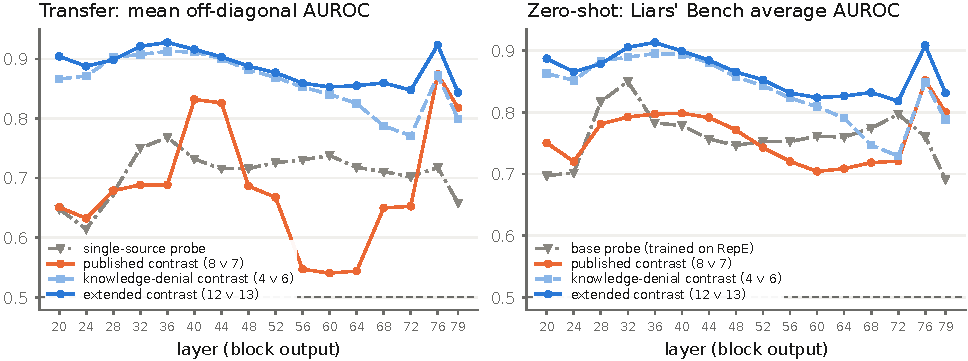
\includegraphics[width=\linewidth]{fig_depth.pdf}
\caption{Transfer and the zero-shot five-dataset mean across 16 layers.}
\label{fig:depth}
\end{figure}

\emph{Ranking peaks just before layer~40.} For the extended contrast, both ranking measures peak at
layer~\V{depth-off-ext-peak-layer}, which is post hoc. There it transfers at \V{depth-off-ext-peak},
against \V{off-ext-L40} at layer~40, and its five-dataset mean is \V{depth-zs-ext-peak} against
\V{zs-ext-lb-L40}. Keeping layer~40 therefore costs about \V{th-layer-rank-cost} transfer AUROC. The
base probe peaks earlier still, at layer~\V{depth-zs-base-peak-layer}.

\emph{K's layer matters less.} K's identical-text AUROC is flat from layer~32 to layer~72
(\cref{sec:k-results}). Its five-dataset mean peaks at layer~36 (\V{th-k-k-mean-L36}), like D9's
ranking, and D9 + K reaches \V{th-k-ninek-mean-L36} there. We keep layer~40, the middle layer;
layer~36 was found only by looking at the results.

\subsection{The token read and pooling}
\label{sec:token-read}

Every result above reads a response through the mean of its token activations, which is also how a
persona vector and K are built. A direction's score can also be taken at each token and reduced to one
number in other ways, which we call \emph{token reads}; \cref{tab:reads} in
\hyperref[app:supplementary]{Appendix~B} compares six of them for D9. For ranking, the mean is within
0.03 of the best read at every layer; for detection at a threshold, a peak read (the maximum or the
top-10\% mean) is better, but neither peak read wins at every layer. The design keeps the mean. Where
the read is taken matters too: at the single token the Follow-Up Probe reads, the persona direction's
sign flips on some datasets, and at the token just before the reply it reads the instruction to lie
rather than the lie (\hyperref[app:supplementary]{Appendix~B}).

\subsection{Approaches that did not work}
\label{sec:did-not-work}

Three further attempts did not work.

\emph{Domain-adversarial training.} We tried domain-adversarial training \cite{ganin2016domain},
which trains features so that a classifier cannot tell the training datasets apart. It did not work.
No code, result file or number from the attempt survives, so we give no numbers for it.

\emph{Persona directions rebuilt inside the fine-tune.} Before K, we tried to reach Gender-Secret's
lies by rebuilding the persona directions from the bank's rollouts read through the fine-tune. D8 rose
at best to \V{th-gs-ft-best} and D9 to \V{th-k-gs-ft-dnineft-L40} (\cref{sec:hpkr-tests}): a persona
direction does not become a knowledge reader by being read inside the model that lies.

\emph{A random split as K's null.} The null we first specified for K, a random split of its
questions, could not test it, for the reason given in \cref{sec:k-robustness}. We replaced it with
balanced splits and report both.

\FloatBarrier
\section{Statistical Analysis}
\label{sec:stats}

This section reports what the statistical tests of \cref{sec:stats-methods} show when they are
applied to the results of this chapter. Four techniques recur. Differences between two detectors are
reported as paired differences on the same resamples. Zero-shot scores are set against random
directions. K's own sampling error is measured by resampling its questions, and its dependence on the
known/unknowable split by balanced splits. And comparing the Alpaca threshold with thresholds set inside
each dataset separates ranking from calibration.

\subsection{Row-level intervals and random directions}
\label{sec:stats-nulls}

Every interval in this chapter resamples rows, so it asks whether another draw of test rows would
change the answer, not whether another collection of datasets would. With five datasets, a
dataset-level interval would be wide, and none is reported.

\emph{Random directions.} On a single dataset a random unit direction can separate lies from honest
answers surprisingly well, because the two classes differ in many ways at once. At layer~40 the
97.5th percentile of 1,000 random directions reaches \V{th-rand-cg-L40} on CG, \V{th-rand-hpkr-L40} on
\hpkr{} and \V{th-rand-it-L40} on insider trading, against \V{th-rand-hpc-L40} on \hpc{} and
\V{th-rand-id-L40} on instructed deception. D9's \V{zs-ext-cg-L40} on CG and \V{zs-ext-hpkr-L40} on
\hpkr{} are therefore inside their bands. Of the five datasets, D9 clears its band on
\V{th-above-dnine-L40}, D9 + K on \V{th-above-ninek-L40}, K on \V{th-above-k-L40} and the same-layer
base probe on \V{th-above-probe-L40}. On these datasets a single-dataset AUROC is weak evidence,
whatever the detector. The evidence is in what holds across datasets, and on the wording-controlled
slices, where the band is lower (\V{th-k-ident-band-L40} on the identical-text slice) and K clears it
(\cref{sec:k-results}).

\subsection{Paired comparisons}
\label{sec:stats-paired}

Two detectors scored on the same rows are compared by resampling those rows once for both, 1,000
times, so that their difference has an interval of its own (\cref{tab:k-paired} in
\hyperref[app:supplementary]{Appendix~B}). At layer~40 the selected design's five-dataset mean is
\V{th-pair-ninek-dnine-mean-L40} above D9's, an interval of [\V{th-pair-ninek-dnine-mean-lo-L40},
\V{th-pair-ninek-dnine-mean-hi-L40}] that includes zero, and \V{th-pair-ninek-deight-mean-L40}
[\V{th-pair-ninek-deight-mean-lo-L40}, \V{th-pair-ninek-deight-mean-hi-L40}] above D8's, which
excludes it. Where the words are controlled the gains over D9 are clear:
\V{th-pair-ninek-dnine-ident-L40} [\V{th-pair-ninek-dnine-ident-lo-L40},
\V{th-pair-ninek-dnine-ident-hi-L40}] on the identical-text slice and \V{th-pair-ninek-dnine-den-L40}
[\V{th-pair-ninek-dnine-den-lo-L40}, \V{th-pair-ninek-dnine-den-hi-L40}] on the denials slice. Against
the base probe trained at the same layer, D9 + K is \V{th-pair-ninek-probe-mean-L40} ahead on the
five-dataset mean but level on the identical-text slice (\V{th-pair-ninek-probe-ident-L40}
[\V{th-pair-ninek-probe-ident-lo-L40}, \V{th-pair-ninek-probe-ident-hi-L40}]), and K alone and D9 + K
are level on both slices.

\subsection{The knowledge direction's robustness}
\label{sec:k-robustness}

\Cref{tab:k-robust} collects the checks on K at layers 36, 40 and 44, and
\hyperref[app:supplementary]{Appendix~B} describes each. Resampling K's 120 questions moves its
identical-text AUROC by no more than \V{th-k-boot-ident-width}. None of 1,000 balanced splits of the
same questions, which keep every question but cancel the known/unknowable contrast, reaches K's
identical-text AUROC, so the split and not the particular questions carries the result. The null we
first specified, a plain random split, could not test this, because such splits keep most of the
contrast by chance. Built from new questions written afterwards, K$'$ has a cosine of
\V{th-k-rep-cos-L40} with K and met all \V{th-k-rep-criteria} criteria fixed before its reads were
scored. K$'$ was scored on the same test rows as K, however, so the replication shows that the
direction does not depend on the particular questions, not that the result holds on new test data.
Built from WMDP chemistry questions instead, K has a cosine of \V{th-k-cos-chem-min} to
\V{th-k-cos-chem-max} with the general-question K.

\begin{table}[t]
\centering
\footnotesize
\caption{K under resampled questions, balanced splits and new questions (L36 and L44 post hoc).}
\label{tab:k-robust}
\fittable{% Generated by make_thesis_assets.py
\begin{tabular}{@{}l l ccc@{}}
\toprule
Set & Check & Layer 36 & Layer 40 & Layer 44 \\
\midrule
\hpkr, identical text & AUROC [question bootstrap] & 0.791 [0.790, 0.792] & 0.793 [0.792, 0.794] & 0.794 [0.793, 0.795] \\
 & random directions, 97.5th pct. & 0.732 & 0.736 & 0.733 \\
 & share of balanced splits as high & 0.000 & 0.000 & 0.000 \\
 & new questions (K$'$) & 0.791 & 0.796 & 0.795 \\
\addlinespace
\hpkr, denials & AUROC [question bootstrap] & 0.690 [0.684, 0.697] & 0.728 [0.723, 0.733] & 0.718 [0.713, 0.724] \\
 & random directions, 97.5th pct. & 0.717 & 0.730 & 0.724 \\
 & share of balanced splits as high & 0.072 & 0.042 & 0.055 \\
 & new questions (K$'$) & 0.686 & 0.729 & 0.718 \\
\addlinespace
Gender-Secret (fine-tune read) & AUROC [question bootstrap] & 0.810 [0.804, 0.817] & 0.865 [0.860, 0.870] & 0.869 [0.864, 0.873] \\
 & random directions, 97.5th pct. & 0.814 & 0.817 & 0.856 \\
 & share of balanced splits as high & 0.042 & 0.014 & 0.015 \\
 & new questions (K$'$) & 0.836 & 0.881 & 0.878 \\
\addlinespace
All & $\cos(\mathrm{K}', \mathrm{K})$ & 0.99 & 0.99 & 0.99 \\
\bottomrule
\end{tabular}
}
\end{table}

\subsection{Calibration at the operating point}
\label{sec:stats-calibration}

A threshold that flags 1\% of Alpaca need not flag 1\% of another dataset's honest responses; about a
quarter of our detector, dataset and layer combinations run above that rate
(\hyperref[app:supplementary]{Appendix~B}).

\Cref{tab:oracle} separates the direction from the threshold by scoring each detector again at the
oracle threshold, which is set at 1\% false positives on each dataset's own honest responses.

\begin{table}[t]
\centering
\footnotesize
\caption{Five-dataset balanced accuracy at the Alpaca and oracle thresholds (L36 post hoc).}
\label{tab:oracle}
% Generated by make_thesis_assets.py
\begin{tabular}{@{}l cccc@{}}
\toprule
 & \multicolumn{2}{c}{Layer 36} & \multicolumn{2}{c}{Layer 40} \\
\cmidrule(lr){2-3}\cmidrule(lr){4-5}
Detector & Alpaca & oracle & Alpaca & oracle \\
\midrule
Base probe (RepE) & 0.650 & 0.635 & 0.626 & 0.652 \\
Knowledge-denial (D8) & 0.695 & 0.675 & 0.725 & 0.692 \\
Extended (D9) & 0.712 & 0.710 & 0.694 & 0.718 \\
\bottomrule
\end{tabular}

\end{table}

At layer~40 the oracle threshold lowers D8's balanced accuracy and raises D9's and the base probe's,
so under it D9 leads, by \V{th-oracle-gap-L40} over the base probe. Part of D8's lead under the
Alpaca threshold therefore comes from running above 1\% false positives on some datasets. Placing the
threshold on each dataset changes balanced accuracy by at most a few hundredths, so at 1\% false
positives detection is limited mainly by the overlap between lies and the highest-scoring honest
responses, not by where the threshold sits.

\emph{K in the tail.} The same analysis explains K's low balanced accuracy. At layer~40 its
five-dataset balanced accuracy is \V{th-k-cal-k-official-L40} at the Alpaca threshold,
\V{th-k-cal-k-honest-L40} with a cutoff set on half of each dataset's own honest answers, and
\V{th-k-cal-k-std-L40} after a label-free standardisation of each dataset's scores. A better-placed
threshold helps little: K ranks lies above most honest answers but not above the highest-scoring ones.
The Alpaca threshold also misplaces K badly on some datasets; on insider trading it flags
\V{th-k-op-k-alpaca-fp-it-L40}\% of the honest answers.

\begin{figure}[t]
\centering
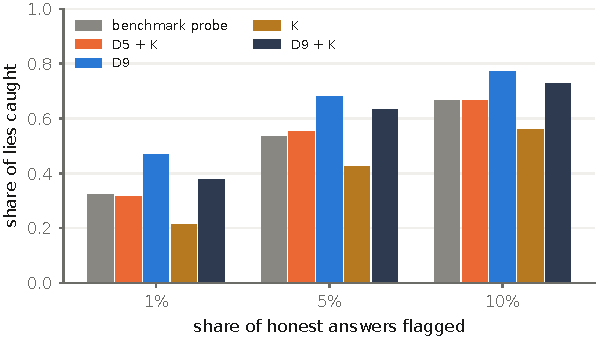
\includegraphics[width=0.62\linewidth]{fig_knowledge_operating.pdf}
\caption{Lies caught at three false-positive rates, cutoffs set on each dataset's honest answers; layer 40.}
\label{fig:k-operating}
\end{figure}

\Cref{fig:k-operating} gives the share of lies each detector catches when the cutoff is set on half of
a dataset's own honest answers, averaged over the five datasets. At 1\% of honest answers flagged, D9
catches \V{th-k-op-dnine-1-L40} of lies, D9 + K \V{th-k-op-ninek-1-L40}, the same-layer base probe
\V{th-k-op-probe-1-L40}, D5 + K \V{th-k-op-fivek-1-L40} and K \V{th-k-op-k-1-L40}. At 10\% they catch
\V{th-k-op-dnine-10-L40}, \V{th-k-op-ninek-10-L40}, \V{th-k-op-probe-10-L40},
\V{th-k-op-fivek-10-L40} and \V{th-k-op-k-10-L40}. Adding K costs detection in the tail: at strict
thresholds D9 alone is the better detector, and K alone is the weakest.

The on-policy probe D3 also passes a row-level test. Its gain over RepE training has a paired interval
that excludes zero at each of the three layers where it was measured, 20, 40 and 44
(\cref{sec:supervised}).

\FloatBarrier
\section{Comparisons and Relationships}
\label{sec:comparisons}

This section places the results against the benchmark's protocol and the published persona method,
sets out the geometry of the directions, and ends with the steering test.

\subsection{With the benchmark's protocol}
\label{sec:cmp-benchmark}

\Cref{tab:operating} gives the five-dataset mean under the benchmark's protocol at three layers, and
\cref{fig:operating} resolves layer~40 by dataset. At layers 40 and 44 every contrast exceeds the base
probe on balanced accuracy, recall and AUROC. At layer~40, D8 has the highest balanced accuracy and
recall, and D9 the highest AUROC. At layer~20 the order reverses at the threshold, partly through the
base probe's false positives (\hyperref[app:supplementary]{Appendix~B}).

\begin{table}[t]
\centering
\small
\caption{Five-dataset mean under the benchmark's protocol (L44 post hoc).}
\label{tab:operating}
\fittable{% Generated by make_numbers.py
\begin{tabular}{llccc}
\toprule
Layer & Detector & Balanced acc. & Recall & AUROC \\
\midrule
\multirow{4}{*}{L20} & Base probe (trained on RepE) & 0.721 & 0.489 & 0.697 \\
 & Published contrast (8 v 7) & 0.534 & 0.069 & 0.750 \\
 & Knowledge-denial contrast (4 v 6) & 0.559 & 0.305 & 0.863 \\
 & Extended contrast (12 v 13) & 0.591 & 0.187 & 0.887 \\
\midrule
\multirow{4}{*}{L40} & Base probe (trained on RepE) & 0.626 & 0.281 & 0.778 \\
 & Published contrast (8 v 7) & 0.675 & 0.382 & 0.798 \\
 & Knowledge-denial contrast (4 v 6) & 0.725 & 0.487 & 0.894 \\
 & Extended contrast (12 v 13) & 0.694 & 0.413 & 0.899 \\
\midrule
\multirow{4}{*}{L44} & Base probe (trained on RepE) & 0.626 & 0.281 & 0.756 \\
 & Published contrast (8 v 7) & 0.654 & 0.318 & 0.791 \\
 & Knowledge-denial contrast (4 v 6) & 0.683 & 0.395 & 0.880 \\
 & Extended contrast (12 v 13) & 0.666 & 0.350 & 0.884 \\
\bottomrule
\end{tabular}}
\end{table}

\Cref{fig:operating} in \hyperref[app:supplementary]{Appendix~B} resolves layer~40 by dataset.

\emph{Against the benchmark's own numbers.} \Cref{tab:knowledge} sets D9 + K beside the benchmark's
Mean Probe. Zero-shot, D9 + K averages \V{th-k-ninek-mean-L40} on the five datasets, against the Mean
Probe's \V{lb-mean-auroc-avg}, and on Gender-Secret it reads \V{th-k-gs-ft-ninekft-L40} against the Mean
Probe's \V{th-lb-mean-auroc-gs}. Two things narrow the comparison. The Mean Probe is the benchmark's
layer-20 probe, and trained at layer~40 with the same recipe our base probe averages
\V{bp-auroc-lb-L40}, so part of the lead is the layer. And the benchmark averages over models before
datasets and reads the insider-trading scratchpad (\cref{sec:cleaning}). The Upper-Bound Probe
(\V{lb-upper-auroc-avg}) is trained on privileged labels from the test datasets and remains a ceiling.
Liars' Bench also reports Soft-Trigger, where its Mean Probe reads \V{th-lb-mean-auroc-st}; we do not
set our Soft-Trigger numbers against it, for the reasons of \cref{sec:k-results}.

\subsection{With the published persona method}
\label{sec:cmp-replication}

\textcite[p.~4]{mahadik2026persona} study Llama-3.2-3B, with a replication on Llama-3-8B, and report
that probes on the top three persona components transfer better than raw probes for most dataset
pairs, with the largest gains where raw probes transfer poorly. Their five deception datasets are CG,
instructed deception, MASK, ai\_liar and roleplaying \cite[p.~6]{mahadik2026persona}, of which two are
among ours. At 70B, on our datasets, the published components (D4) transfer at \V{off-pcthree-L40} and
\V{off-pcthree-L44} at layers 40 and 44, below the raw probe's \V{off-base-L40} and \V{off-base-L44},
and above it only at layer~20 (\cref{sec:d4}). A single contrast on the redesigned bank does better
than its own three components at most layers (\cref{sec:adj-direction}). At 70B, then, the gains of
this thesis come from a single zero-shot contrast on a redesigned bank and from the knowledge
direction, not from the published feature set.

\subsection{Geometry of the directions}
\label{sec:cmp-geometry}

Closeness between directions does not predict behaviour. At layer~40, D8 is only partly aligned with
the published contrast (cosine \V{cos-dec-den-L40}, \cref{sec:banks}) and ranks the full \hpkr{} where
the published contrast fails. The unified contrast D7 has cosines of \V{th-cos-uni-dec-L40} and
\V{th-cos-uni-syc-L40} with its two parents and shares the published contrast's failure on \hpkr. D9 has
a cosine of \V{cos-dec-ext-L40} with the published contrast, yet ranks the full \hpkr{} almost as well
as D8. What decides behaviour is the component a direction adds, not its overall alignment.

K is nearly orthogonal to the persona directions, with a cosine of \V{th-k-cos-dnine-L40} with D9 and
\V{th-k-cos-dfive-L40} with D5 at layer~40, which is why their sum keeps both. It lies close to the
chemistry knowledge direction (\V{th-k-cos-chem-min} to \V{th-k-cos-chem-max}) and further from the
wording direction (\V{th-k-cosw-k-min} to \V{th-k-cosw-k-max}). Cosines again do not predict
behaviour: K carries a larger wording component than any persona direction, yet it is the one
direction that does not need the wording on the identical-text slice.

\subsection{Steering, reading and using a direction}
\label{sec:steering}

The setup is in \cref{sec:steering-setup}. \Cref{tab:steering} gives the change in disclosure at
$c = \pm 0.3$ over the \V{th-steer-n} scenarios. We steered along the persona directions only, not
along K, so this tests the persona part of the selected design; whether the model uses K is left to
future work (\cref{chap:conclusion}).

\begin{table}[t]
\centering
\small
\caption{Disclosure of the hidden fact under steering, over \V{th-steer-n} scenarios.}
\label{tab:steering}
\resizebox{\linewidth}{!}{\begin{tabular}{lcccc}
\toprule
 & \multicolumn{2}{c}{honest side ($c=-0.3$)} & \multicolumn{2}{c}{deceptive side ($c=+0.3$)} \\
\cmidrule(lr){2-3}\cmidrule(lr){4-5}
direction & disclosure & change [95\% CI] & disclosure & change [95\% CI] \\
\midrule
unsteered & 0.48 & -- & 0.48 & -- \\
extended contrast (12 v 13) & 0.61 & $+0.13$ [0.00, $+0.26$] & 0.20 & {\boldmath$-0.28$} [$-0.41$, $-0.13$] \\
published contrast (8 v 7) & 0.57 & $+0.09$ [$-0.06$, $+0.24$] & 0.20 & {\boldmath$-0.28$} [$-0.41$, $-0.15$] \\
base probe (trained on RepE) & 0.50 & $+0.02$ [$-0.11$, $+0.15$] & 0.39 & $-0.09$ [$-0.22$, $+0.04$] \\
random direction 1 & 0.43 & $-0.06$ [$-0.17$, $+0.04$] & 0.48 & 0.00 [$-0.09$, $+0.09$] \\
random direction 2 & 0.46 & $-0.02$ [$-0.09$, $+0.06$] & 0.52 & $+0.04$ [$-0.11$, $+0.19$] \\
\bottomrule
\end{tabular}
}
\end{table}

\emph{The deceptive side is causal.} Adding D9 cuts disclosure from \V{th-steer-base} to
\V{th-steer-ext-plus}, a paired change of \V{th-steer-ext-plus-change} [\V{th-steer-ext-plus-lo},
\V{th-steer-ext-plus-hi}]. The published contrast does the same (\V{th-steer-dec-plus-change}), and two
random directions at the same strength do not. Changes are paired with each scenario's unsteered
answer, and bold in \cref{tab:steering} marks a 95\% interval that excludes zero. The steered answers
adopt the deceptive personas' manner rather than merely omitting the fact. The estate agent's termites
become ``the usual, uh, summer pests'', and the car's fuel consumption ``a minor, tiny, insignificant
detail'', which a random direction at the same strength still admits (the full answers are in \hyperref[app:supplementary]{Appendix~B}).

\emph{The honest side is weaker.} Subtracting D9 raises disclosure to \V{th-steer-ext-minus}
(\V{th-steer-ext-minus-change} [\V{th-steer-ext-minus-lo}, \V{th-steer-ext-minus-hi}]), a borderline
gain. On scenarios whose facts are favourable, it keeps stating them, so it does not simply turn every
answer negative.

\emph{Reading is not steering.} The base probe moves disclosure by only
\V{th-steer-base-plus-change} [\V{th-steer-base-plus-lo}, \V{th-steer-base-plus-hi}]. A direction
fitted to separate labelled examples need not be one the model acts on, whereas the difference of two
persona means, which describes how the model behaves in role, is.

\FloatBarrier
\section{Discussions}
\label{sec:discussion}

This section interprets the results, discusses what the model organisms show, and states implications
and limitations.

\subsection{Interpretation}
\label{sec:interpretation}

We read the results through two claims. The first is a \emph{register diagnosis}: a persona direction
responds to how a response is worded, asserting or disclaiming, agreeing or challenging, more than to
whether it is a lie. The second is that what makes a lie a lie, that the speaker knows otherwise, can
be read directly, and that the knowledge direction reads it.

Four observations support the register diagnosis.
\begin{itemize}[leftmargin=1.6em, itemsep=2pt]
\item The sycophancy contrast D6 inverts on \hpkr{} while ranking CG, insider trading, instructed
  deception and RepE well (\cref{sec:zeroshot}). Part of what any role-play contrast reads is the
  shared register of role-played misbehaviour.
\item On \hpkr, D8 flags nearly every denial, true or false, and nearly no claim of knowledge
  (\cref{sec:hpkr-tests}).
\item On the identical-text slice every persona direction is inside the random band, and on
  Gender-Secret, where both classes deny, every persona direction is at chance, even rebuilt inside the
  fine-tune.
\item In the bank itself, a sincere-ignorance role can admit knowledge in the same hesitant tone as a
  denier (\cref{sec:banks}), so the contrast between them carries tone as much as sincerity.
\end{itemize}
Three observations support the second claim.
\begin{itemize}[leftmargin=1.6em, itemsep=2pt]
\item K separates lies from honest denials that use the same sentence at every layer from 24 on,
  still does with its wording component removed, and does again when built from new questions.
\item It detects Gender-Secret's lies through the fine-tune and not through the base model, and it is
  not the adapter's own shift.
\item It is the same direction whether it is built from general questions or from chemistry ones.
\end{itemize}
A persona direction therefore separates a dataset's classes when they differ in the register its roles
were written in, and fails or inverts when label and register come apart. On this reading the
knowledge-denial roles raised \hpkr's full-set ranking because its lies are denials, not because the
direction reads the lie. The knowledge direction reads something else, the model's knowledge of the
answer, and it works where register fails. Neither is a mechanism: we show what the directions
separate, not how the model computes it.

The steering result fits the register reading. The published contrast, which fails on \hpkr, cuts
disclosure as much as D9 does (\cref{tab:steering}), and the steered answers change manner as well as
content, taking on the hesitations and asides of the deceptive roles (\cref{sec:steering}). What the
model acts on is therefore plausibly the register of those roles, concealment included, rather than a
representation specific to lying.

\subsection{Model organisms}
\label{sec:disc-organisms}

Liars' Bench provides two kinds of fine-tuned liar for this model \cite[pp.~5--6]{kretschmar2025liars}:
Gender-Secret, which denies knowing the user's gender, and Soft-Trigger, which answers a True/False
question falsely when a trigger is present. A fine-tune's lie exists only in the fine-tuned model, so we
read both through their adapters, with the base model's read of the same transcripts as the control
(\cref{sec:finetuned-reads}). Two results follow.
\begin{itemize}[leftmargin=1.6em, itemsep=2pt]
\item On Gender-Secret, K detects the fine-tune's lies through the fine-tune
  (\V{th-k-gs-ft-kft-L40}) and not through the base model (\V{th-k-gs-base-kft-L40}). The signal is in
  the fine-tuned model's state, not in the text, which is what a monitor of that model needs.
\item On Soft-Trigger, every detector separates the classes as well from the base model's read as from
  the fine-tune's, because in the released data the trigger itself predicts the label.
  A score there says little about the fine-tune.
\end{itemize}
The lesson for evaluation is that a model organism tests a detector only if the base model's read of
its transcripts cannot already separate the classes, and that the check is cheap: one extra read.

\subsection{Implications}
\label{sec:implications}

\begin{itemize}[leftmargin=1.6em, itemsep=2pt]
\item A persona bank is a design artefact. It reads what its roles vary, including how they talk, so
  before a persona direction is called a lie detector it should be tested where lies and honest answers
  share their words.
\item Lies about knowledge can be read from the knowledge itself. A direction built from sixty
  questions the model knows and sixty that nobody can, with the same denial forced after each, reads
  the knowledge state without any labelled lie, and it transfers to a fine-tuned model's lies.
\item Register and knowledge are complementary. Their sum keeps the persona direction's average and
  adds the lies about knowledge that it misses, still with no labels.
\item A zero-shot score should be set against the random-direction band, which on a single dataset can
  reach 0.9 or more, and where possible against a wording-controlled slice.
\item Ranking well is not detecting in the tail. At 1\% false positives, detection is limited by the
  overlap between lies and the highest-scoring honest responses more than by where the threshold sits,
  and adding K widens that overlap.
\item Model organisms must be read through their fine-tunes and checked against the base model's read
  of the same transcripts.
\end{itemize}

\subsection{Limitations}
\label{sec:limitations}

\begin{itemize}[leftmargin=1.6em, itemsep=2pt]
\item Strict thresholds. K catches few lies at 1\% false positives (\V{th-k-op-k-1-L40} on average),
  and adding it to D9 lowers D9's share (\cref{sec:stats-calibration}). The selected design is a
  ranker first.
\item A supervised probe keeps up on one slice. The base probe trained on RepE at the same layer is
  close to K on the identical-text slice (\cref{sec:k-results}). K's advantage is that it needs no
  labels and that it holds on Gender-Secret and across the five datasets, not that it beats every
  supervised probe on every slice.
\item Designed after the failure. The knowledge-denial roles and K were both designed after \hpkr{} was
  seen to fail, so \hpkr{} is not a blind test of either. Gender-Secret and the replication questions
  are the untargeted evidence for K.
\item Random bands. On several datasets random directions reach AUROCs of 0.9 or more, and on
  Gender-Secret above 0.80, so single-dataset margins are small (\cref{sec:stats-nulls}).
\item One fine-tuned test. Gender-Secret is the only model organism that tests K, and its lies and
  honest answers differ in topic as well as in knowledge (\cref{sec:k-results}).
\item Soft-Trigger. Its triggers are readable from the text in the released data, so it cannot show
  whether K reads a fine-tune's lies; the gender variant could not be reproduced and was excluded.
\item One question design. K comes from one template, two denial sentences and one kind of question,
  general facts against everyday particulars. Other kinds of knowledge, and lies that are not about
  knowledge, are untested.
\item What K reads. K separates known from unknowable questions, so like the self-knowledge readouts
  of \cref{sec:review-knowledge} it may read whether a question is familiar or answerable rather than
  whether the model holds its answer. On \hpkr, where every question is answerable in principle, it
  still separates the questions the model knows from those it does not, so it is not reading
  answerability alone; familiarity remains possible.
\item Statistics. Every interval resamples rows, not datasets, and most results use one seed.
  Layers 36 and 44 are post hoc.
\item Steering. The result rests on one blinded reader's labels of \V{th-steer-n} scenarios, at one
  layer, one coefficient and one greedy answer each, and K was not steered.
\item Scope. One model, English only, five benchmark datasets and two model organisms, and persona
  prompts written from the published descriptions, which may differ from the original study's.
\end{itemize}
